\documentclass[a4paper]{article}

\usepackage{amsmath}
\usepackage{amssymb}
\usepackage{parskip}
\usepackage{fullpage}
\usepackage{hyperref}
\usepackage{xcolor}
\usepackage{stellar}
\usepackage{chronology}
\usepackage{tikz}
\usepackage{fancybox}
\usepackage{makecell}
\usepackage{bettelini}

\hypersetup{
    colorlinks=true,
    linkcolor=black,
    urlcolor=blue,
    pdftitle={Storia},
    pdfpagemode=FullScreen,
}

\title{Storia}
\author{Paolo Bettelini}
\date{}


\begin{document}

\maketitle
\tableofcontents
\pagebreak

% EAN 9788859300434

\section{Storia}

\sdefinition{Storiografia}{
  La \textit{storiografia} è la disciplina scientifica che si occupa di studiare la storia.
}

\section{Periodizzazione}

\sdefinition{Periodizzazione}{
  La \textit{periodizzazione} è l'operazione culturale volta a suddividere la linea temporale in vari intervalli,
  ciascuno con caratteristiche comuni.
}

Le prime periodizzazioni derivano dalle prime religioni monoteiste (Es. nascità di Gesù, calendario islamico).

Le periodizzazioni sono delle convenzioni.

\section{Fake news storiche}

% Da: Fascismo e fake news

Le fake news sono in genere effimere, ma quelle storiche sono persistenti e
pronfonde nelle persone.

\begin{itemize}
    \item Più una bugia viene ripetuta, più la si può scambiare per verità.
    \item Notizie di oggi viaggiano velocemente, è difficile bloccarle e smentirle.
    \item Comprendere il passato è un modo per comprendere il presente.
    \item Esistono fake news storiche, ancorate ad un argomento preciso.
    \item Bufale storiche vanno contrastate perché falsificano il passato (così come il ricordo e la memoria).
    \item Bufale storiche nascono da osservazioni o testimonianze inesatte, che poi si diffondono in una società pronta ad accoglierle.
    \item Bufale storiche servono ad alimentare emozioni e a rassicurare: credere in un passato positivo può portare la speranza e rischia di creare una prospettiva a cui tendere.
\end{itemize}

Effetti di scardinare le bufale:

\begin{itemize}
    \item Corregere le informazioni sul passato.
    \item Distruggere sicurezze, e ciò può creare incomunicabilità.
    \item Permette di limitare l'ambito di diffusione di queste notizie, che mistificano la memoria e la percezione del presente.
\end{itemize}

\pagebreak

\section{Linea temporale}

\begin{chronology}[250]{-1251}{2010}{\textwidth}
    \event{-1250}{Caduta di Troia}
    \event{-753}{Romolo Re di Roma}
    \event{1}{Nascita di Gesù}
    \event{622}{Egira}
    \event{800}{Carlo Magno Imperatore}
    % rinascimento
    %\event[1450]{1700}{Rinascimento}
    \event{1517}{Riforma protestante}
    % illuminismo
    \event{1789}{Rivoluzione francese}
    % romanticismo
    \event{1922}{Marcia su Roma}
\end{chronology}

\begin{chronology}*[500]{-3000}{2010}{\textwidth}
    \event{476}{Crollo Impero Romano d'Occidente}
    \event{1453}{Crollo Impero Romano d'Oriente}
    \event[-3000]{476}{Età antica}
    \event[476]{1492}{Medioevo}
    \event[1492]{1789}{Età moderna}
    \event[1789]{2010}{Età contemporanea}
\end{chronology}

% preistoria - fino a -3000

\section{Fonti}

Le fonti possono essere distinti in
\begin{itemize}
    \item \textbf{Fonti materiali:} oggetti e i reperti storici.
    \item \textbf{Fonti scritte:} scritto su carta o altri materiali storici.
    \item \textbf{Fonti figurate o iconografiche:} immagini che rappresentano eventi o scene del passato.
    \item \textbf{Fonti orali:} racconti delle persone presenti a un avvenimento.
\end{itemize}

% volontarie e involontarie, dirette indirette

\pagebreak

\section{Antico Regime}

\sdefinition{Antico Regime}{
    Una società dominata dalla disuguaglianza e dall'ingiustizia.
    Antico regime è il termine con il quale gli storici indicano l'insieme delle istituzioni
    politiche, giuridiche, economiche e sociali caratteristiche di gran parte dell'Europa tra 16°
    e 18° secolo. L'espressione ancien régime ("antico regime") fu introdotta dai rivoluzionari
    francesi del 1789 per contrapporre il vecchio regime prerivoluzionario al nuovo regime da
    loro creato in Francia con la Rivoluzione francese.
}

L'Antico regime era un tipo di società caratterizzata:
\begin{itemize}
    \item dall'autorità di un sovrano assoluto alleato con un una Chiesa
        intollerante;
    \item dal diritto fondato sulle disuguaglianze di nascita, che non
        riconosceva il valore del merito e della competenza;
    \item da un ordinamento oppressivo che imponeva ai contadini le
        servitù personali e che in generale schiacciava i sudditi sotto il
        peso delle tasse.
\end{itemize}

L'antico regime è difficile da periodizzare perché è composto da diverse
componenti di diverse epoche, anche di milleni di anni, ancora rigorosamente in vigore.

\subsection{Monarchia}

\sdefinition{Monarchia}{
    Forma di governo in cui i supremi poteri dello stato sono
    accentrati in una sola persona (re, sovrano, monarca), la cui carica non è elettiva e che può
    essere anche affiancata da altre istituzioni: m. \textit{Ereditaria}, \textit{non ereditaria}; m. \textit{Assoluta}, in
    cui il supremo governo statale è concentrato nel monarca; m. \textit{Limitata} o \textit{costituzionale},
    quando, accanto al monarca, vi sono altre istituzioni sovrane, quali il parlamento e il
    governo, che ne controllino il potere in base a una costituzione: si distingue
    la m. \textit{Costituzionale parlamentare} dalla m. \textit{Costituzionale pura} secondo che sia o no in
    vigore il principio parlamentare, ossia della necessità di un rapporto di fiducia fra
    esecutivo e legislativo.
}

Un uomo detenie quindi la sovranità, affidatagli generalmente da una divinità
per guidare il popolo verso la prosperità (legittimazione divina del potere).
La carica è ereditaria e a vita.
Nelle monarchie assolute il potete è indivisibile, è tutto nelle mani
della medesima persona.

\subsection{Repubblica}

\sdefinition{Repubblica}{
    Con riferimento all'età classica, al
    medioevo e alla prima età moderna, ogni stato non retto da un monarca o da un
    dittatore: la R. romana o di Roma, dal 509 al 31 a. C.; le r. oligarchiche della Grecia; le
    R. marinare italiane; la R. di Cromwell in Inghilterra (metà del sec. 17°), ecc. 
}

Una parte dei cittadini detiene la sovranità, che viene esercitata entro i limiti stabiliti dalle leggi.
Vi è una presenza di una pluralità di istituzioni.
La carica pubblica non è ereditaria e generalmente limitata nel tempo.\\
\textbf{\color{red}nota:} una repubblica non è necessariamente democratica.

\subsection{Impero}

\sdefinition{Impero}{
    Per impero si intende un organismo politico costituito da diversi paesi, popolazioni e Stati
collocati anche in zone non contigue, in molti casi caratterizzato dalla presenza di razze
diverse e culture e lingue non omogenee, ma sempre dotato di un centro politico e di un
nucleo nazionale dominante che esercita sull'insieme il comando e il potere supremo.
Nell'antichità e nel Medioevo a capo degli imperi vi erano i monarchi, mentre in età
moderna e contemporanea imperi sono state anche alcune repubbliche.[…]
Il maggiore e più durevole impero del mondo antico sorto in Occidente fu quello romano,
le cui origini vanno ricondotte all'opera dell'imperatore Augusto a partire dal 27 a.C.: egli
riordinò i grandi territori già conquistati da \href{http://www.treccani.it/enciclopedia/roma_(Enciclopedia_dei_ragazzi)/}{Roma} in età repubblicana, territori che
sarebbero stati ulteriormente accresciuti dai suoi successori in Europa, Asia e Africa. I
fondamenti della politica imperiale furono la superiorità militare dei Romani, una
crescente uniformità amministrativa, la diffusione della cultura greco-latina come cultura
egemone, l'allargamento della cittadinanza.\\
Data la sua estensione, l'Impero venne diviso tra il 3° e il 4° secolo in una parte occidentale
e in una parte orientale. Nel 4° secolo l'Impero divenne ufficialmente cristiano
e \href{http://www.treccani.it/enciclopedia/costantino-i-il-grande_(Enciclopedia_dei_ragazzi)/}{Costantino} spostò la capitale principale da Roma a Costantinopoli. Nel 476 l'Impero
d'Occidente crollò in seguito alle invasioni barbariche, mentre quello d'Oriente, l'\href{http://www.treccani.it/enciclopedia/impero-bizantino_(Enciclopedia_dei_ragazzi)/}{Impero bizantino},
sopravvisse fino al 1453, quando venne definitivamente abbattuto dai Turchi
ottomani.
}

\begin{itemize}
    \item Generalmente comprende vasti territori e popoli diversi, soggetti ad un'unica autorità che garantisce l'equilibrio tra le varie componenti territoriali ed etniche;
    \item sono possibili modalità di nomina diverse per l'imperatore: elezione, designazione, ereditarietà;
    \item un impero si fonda su un'ideologia a carattere universale, ovvero ha l'ambizione di costruire l'unica civiltà esistente (o comunque una civiltà superiore).
\end{itemize}

\subsection{Monarchia feudale}

\sdefinition{Feudo}{
    Grossa proprietà terriera
}

\sdefinition{Monarchia feudale}{
    Stato di proprietari, legati da un rapporto personale di subordinazione verso il sovrano che aveva donato loro la terra, e, con la terra, l'autorità.
}

In una monarchia feudale il potere del sovrano è limitato:
\begin{itemize}
    \item Non possiede una forza militare (diretta). La forza militare è quella dei feudatari che fanno giuramento verso il re;
    \item ha un potere fiscale ridotto;
    \item l'amministrazione del terrotorio e della giustizai è delegata ai signori, nobili feudatari, vassalli del re;
    \item il clero (la Chiesa) amministra le proprie terre;
    \item i comuni con status particolari (non sono sotto diretto potete del sovrano).
\end{itemize}

\sdefinition{Stato}{
    Entità giuridica dotata del monopolio amministrativo,
    giudiziario, politico e coercitivo in un determinato
    territorio, coeso e munito di precise frontiere.
}

Lo stato è quindi un territorio con dei cittadini ed un governo.

Lo stato può essere:
\begin{itemize}
    \item Autoritario (Es. Cina, Corea del Nord)
    \item Liberale/Democratico (Es. Svizzera)
    \item Unitario/Centralistico (Es. Italia, Monarchia che centra il potere)
    \item Federale (Es. Svizzera)
    \item Confederali (Es. ex Svizzera, Germania)
    \item Confessionale (Es. Vaticanow, Iran)
    \item Laico (non confessionale)
    \item Socialista (Es. Cina, Cuba, Corea del Nord)
    \item Capitalista
\end{itemize}

\sdefinition{Stato Moderno}{
    Lo \textit{stato moderno} è sorto in Europa
    tra il 15° e il 16° secolo, trovando la sua espressione dominante nella monarchia assoluta, che
    a partire dalle grandi monarchie nazionali di Spagna, Inghilterra e Francia pose gradualmente
    fine al particolarismo di matrice feudale o quanto meno lo ridusse fortemente ponendolo
    sotto il proprio controllo.
}

I suoi membri - individui e organismi collettivi - sono sottomessi unicamente alla legge,
garanzia dei diritti statuiti e sottoposti al controllo dell'ordine giudiziario.

Il primo tipo di stato è stato lo stato moderno, che poi si è trasformato in stato liberale democratico
nei tempi moderni.
Vi sono principalmente tre fattori che hanno procurato il passaggio da monarchia feudale a stato moderno:

\begin{itemize}
    \item
    Il passaggio dal Medioevo al Rinascimento ha visto un profondo cambiamento nell'assolutismo, che non era più solo teorico ma divenne effettivo nel Cinquecento e Seicento. Questo cambiamento è attribuibile principalmente alla nuova struttura dello Stato, in particolare all'istituzione di eserciti permanenti che garantivano il potere del re. Questi eserciti, sia sotto forma di guarnigioni fisse che di truppe mobili, erano ora composti da fanterie mercenarie dipendenti solo dal re e non più dalla feudalità. La fanteria, diventata la principale forza militare, consentiva al sovrano di esercitare una politica estera più ampia.
    \item
    Inoltre, si è assistito a un cambiamento nella politica estera con l'organizzazione della prima diplomazia permanente, contrariamente al Medioevo in cui le relazioni internazionali erano meno strutturate. Questo cambiamento ha portato all'idea di equilibrio di potere tra gli Stati europei.
    \item
    Oltre all'esercito e alla diplomazia, la burocrazia statale è emersa come elemento chiave, con una crescente potenza degli "ufficiali"/funzionari del sovrano. In questo periodo, lo Stato si è concentrato attorno al potere sovrano e alla gerarchia degli ufficiali, piuttosto che sugli "ordini" della nazione o gli Stati generali.
    Vendita della cariche.
\end{itemize}

Questi processi mirano i ridurre il potere dei feudali ed aumentare quello del sovrano.

Nel 1685 Luigi XIV comanda tutti gli Ugonotti di convertirsi al cristianesimo creando
un'uniformità religiosa.

Il Re diventato lo Stato sotto tutti gli effetti.

\subsection{La Società dell'Antico Regine}

\begin{center}
    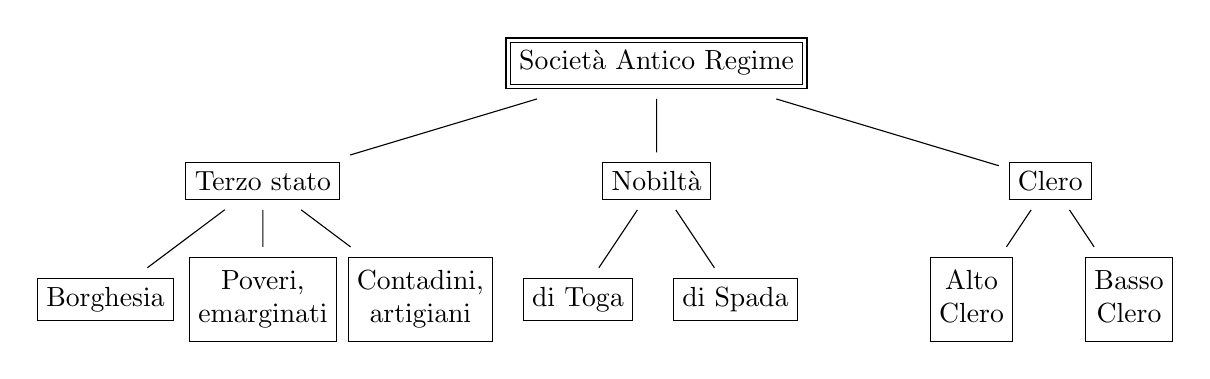
\begin{tikzpicture}[
        level 1/.style = {sibling distance = 5cm},
        level 2/.style = {sibling distance = 2cm}
    ]
    \node {\doublebox{Società Antico Regime}}
        child {
            node {\fbox{Terzo stato}}
            child {
                node {\fbox{Borghesia}}
            }
            child {
                node {\fbox{\makecell[c]{Poveri, \\ emarginati}}}
            }
            child {
                node {\fbox{\makecell[c]{Contadini, \\ artigiani}}}
            }
        }
        child {
            node {\fbox{Nobiltà}}
            child {
                node {\fbox{di Toga}}
            }
            child {
                node {\fbox{di Spada}}
            }
        }
        child {
            node {\fbox{Clero}}
            child {
                node {\fbox{\makecell[c]{Alto \\ Clero}}}
            }
            child {
                node {\fbox{\makecell[c]{Basso \\ Clero}}}
            }
        };
    \end{tikzpicture}
\end{center}

Non si può accedere al clero per nascita.
Le tasse appartengono unicamente a quelli appartenenti al terzo stato.
Non vi è libertà di pensiero, culto o parola.

Questo tipo di società è divisa per discendenza eccetto per il Clero.
Il primo genito di una famiglia nobiliare eredita spesso le varie terre, mentre il secondo genito
andrà a fare parte dell'Alto Clero, mentre il Basso Clero è principalmente occupato dalla Borghesia.

\subsection{Fallimento dell'accentramento monarchico in Inghilterra}

Carlo I Stuart fu il primo sovrano decapitato dal popolo.
Il parlamento in inghilterra non si fa scavalcare, e i sovrani, a differenza di quelli francesi,
non riescono così tanto a centralizzare il potere.
Il parlamento si ribella e obbliga i nuovi sovrani di firmare il "Bill of rights".

\sdefinition{Bill of Rights}{
    Il parlamento impone (non chiede) al sovrano di essere riconosciuto.
}

\begin{itemize}
    \item Il potere limtiato dal re;
    \item un parlamento rappresentativo dotato del monopolio legislativo;
    \item sistenza giudiziario a garanzia dell'integrità delle persone e di alcuni diritti indivuduali
\end{itemize}

Alcuni elementi per essere uno Stato moderno sono assenti, il potere non è infatti centralizzato.
Tuttavia, è uno Stato Moderno perché riconosce i diritti individuali nei confronti del potere dello Stato.
Seppur limitato, il otere del sovrano viene esercitato in modo uniforme su tutti i sudditi e su tutto il territorio.

Il potere statuale non è più concentrato, bensì ripartito tra figure diverse:
\begin{itemize}
    \item il re possiede il potere esecutivo;
    \item il parlamento ha potere legislativo;
    \item giudici hanno potere giudiziario.
\end{itemize}

% TODO stato liberale rappresentativo e le costituzioni
% TODO differenza fra monarchia costituzionale e parlamentare

\subsection{Illuminismo}

\sdefinition{Illuminismo}{
    L'\textit{illuminismo} è una corrente di pensieri anche nominata l'età dei lumi.
    La luce alla quale si fa riferimento è in diretta contrapposizione
    al medioevo e diverse concezioni dell'Antico Regime, ossia, all'ignoranza.
}

L'illuminismo è caratterizzato dall'autonomia dell'individuo e uso della ragione.
Un movimento cosmopolita (La Natura, Il Cosmo sono gli stessi ovunque si metta piedei. Perciò essi
potevano vivere allo stesso modo in accordo con la natura ovunque. Essi non erano a casa in una città
o in un'altra, ma nella natura, nel Cosmo. Si chiamavano infatti cittadini del Cosmo: cosmopoliti).
Inoltre, era caratterizato dalla tolleratanza; libertà di coscienza e di opinione.

% TODO def intolleranza. di alberto pincherie Encliclopedia italiana 1933
Possiamo cominciare a parlare di tolleranza quando vi sono motleplici religioni o teismi che sostengono di possedere la verità assoluta, le quali vanno in conflitto diretto con le altre.

\sdefinition{Giusnaturalismo}{
    Il \textit{giusnaturalismo} è corrente filosofica giuridica, fondata su due principi:
    \begin{itemize}
        \item esiste un diritto naturale (conforme cioè alla natura dell'uomo e quindi intrinsecamente corretto);
        \item è superiore al diritto positivo (diritto prodotto dagli uomini).
    \end{itemize}
}

Esistono norme di diritto naturale che hanno per oggetto la tutela della vita, della libertà e della proprietà.

% ILLUMINISMO E POLITIC
% 3 organi SEPARATI e indipendenti in manira tale che essi si bilancino e si frenino a vicenda.

\end{document}
